
\chapter{数论}
\label{chap:number-theory}

\epigraph{Die ganzen Zahlen hat der liebe Gott gemacht, alles andere ist Menschenwerk.\\
  上帝创造了自然数,其余的都是人的工作。}{Leopold Kronecker(利奥波德·克罗内克)}

Kronecker是德国数学家与逻辑学家,主要研究代数和数论,特别是在椭圆函数理论上有突出贡献。以克罗内克命名的数学理论包括克罗内克$\delta$函数、克罗内克积等。

\section{自然数}
\label{sec:what-is-natural-number}

关于自然数(Natural Number)所指,目前并没有定论,有时是指正整数$1,2,3,\cdots$,有时是指非负整数$0,1,2,3,\cdots$,取决于主观意愿。在这里,为避免混淆,只采用正整数、非负整数等无疑义的说法。

\section{质数}
\label{sec:prime-number}

\begin{definition}[质数,Prime Number]
  一个大于$1$的正整数,若除了$1$和它本身之外没有其它的因子,则称该数为质数,也叫素数。不是质数的正整数称为合数。
\end{definition}

\begin{table}[htbp]
  \centering
  \caption{100以内的质数}
  \label{tab:prime-numbers<100}
  \begin{tabular}{cccccccccc}
    \hline
    2  & 3  & 5  & 7  & 11 & 13 & 17 & 19 & 23 & 29\\
    31 & 37 & 41 & 43 & 47 & 53 & 59 & 61 & 67 & 71\\
    73 & 79 & 83 & 89 & 97 &    &    &    &    &   \\
    \hline
  \end{tabular}
\end{table}

\begin{property}
  $2$是唯一的一个偶数质数。
\end{property}

\begin{theorem}
  有无穷多个质数。
\end{theorem}
\begin{proof}
  下面是欧拉提出的方法,用反证。假设只有有限个质数$p_1,p_2,\cdots,p_n$,那么对于正整数$p_{n+1}=p_1p_2p_3\cdots p_n + 1$,显然有$p_{n+1}$不被$p_1,p_2,\cdots,p_n$整除,从而找到一个$p_1,p_2,\cdots,p_n$之外且比它们都大的质数$p_{n+1}$,矛盾。
\end{proof}

可以用欧拉的反证法构造质数数列。从质数数列$p_1,p_2,\cdots,p_n$出发,则$p_1p_2\cdots p_n+1$要不是质数,要不就含有一个不同于$p_1,p_2,\cdots,p_n$的质因子,从而可找到下一个质数$p_{n+1}$。

\begin{example}
  从$41$出发,按欧拉方法找出$5$个不同的质数。
\end{example}
\begin{proof}[解]千万不要用纸笔算,除非你想锻炼计算能力,请利用计算机编程验证,让合适的人做合适的事。
  \begin{align*}
    p_1 & = 41 && p_1 + 1 = 42 = 2\times 3\times 7&&\text{随便取一个,比如取2}\\
    p_2 & = 2  && p_1p_2 + 1 = 2\times41 + 1=83   &&\text{是质数}\\
    p_3 & = 83 && p_1p_2p_3 + 1=6807=3\times2269  &&\text{为方便起见,取3}\\
    p_4 & = 3  && p_1p_2p_3p_4+1=20419=7\times2917&&\text{取7}\\
    p_5 & = 7  &&                                 &&\qedhere
  \end{align*}
\end{proof}

下面是除了著名的哥德巴赫猜想(参考例~\ref{ex:Goldbach-conjecture})之外的又一个关于质数的悬而未决的猜想。
\begin{example}[成对质数的猜想]
  以$p$与$p+2$形式成对出现的质数有无穷多个。
\end{example}
\begin{proof}[示例]
  如$(3,5)$、$(11,13)$、$(17,19)$、$(29,31)$和$(41,43)$等等都是这种成对形式的质数。
\end{proof}

\section{整除}
\label{sec:divisible}

\begin{definition}
  若整数$a$是整数$b$的整数倍,即存在某个整数$q$,使得$a=bq$,则称$b$整除$a$,也称$a$被$b$整除。记为$b\mid a$。$b$不能整除$a$则记为$b\notdivides a$。
\end{definition}

\begin{example}
  \begin{align*}
    17293\mid 0,\quad 4\mid 28,\quad 5\notdivides 12
  \end{align*}
\end{example}

\subsection{最大公约数}
\label{sec:gcd}

\begin{definition}[最大公约数,Greatest Common Divisor(gcd)]
  两个不同时为零的整数$a,b$的公约数中最大的一个称为$a,b$的最大公约数,记为$\gcd(a,b)$。
\end{definition}

\begin{example}
  \begin{align*}
    \gcd(0,8)=8,\quad 
    \gcd(-9,-12)=\gcd(9,12)=3,\quad
    \gcd(7,22)=1
  \end{align*}
\end{example}

\begin{definition}[互质,Coprime]
  若$\gcd(a,b)=1$,则称$a,b$互质。
\end{definition}
$\gcd(a,b)=1$是指$a,b$除了$1$之外没有其余的正的公约数。

\begin{theorem}
  若$a,b$互质,且质数$p\mid ab$,则必有$p\mid a$或者$p\mid b$。
\end{theorem}
\begin{corollary}
  若$a_1,a_2,\cdots,a_n$两两互质,且质数$p\mid a_1a_2\cdots a_n$,则$p$必能整除$a_1,a_2,\cdots, a_n$中的某一个。
\end{corollary}

\begin{example}
  $4,5,9$两两互质,其乘积为$4\times5\times9=180$,作质因式分解,有
  \begin{align*}
    180=2^2\times 3^2\times 5
  \end{align*}
  从而能整除$180$的质数只有$2,3,5$,这三个数都能整除$4,5,9$中的某一个。
\end{example}

\begin{theorem}
  若整数$a,b$互质,且$b\mid ac$,则必有$b\mid c.$
\end{theorem}

\begin{definition}[欧拉函数,Euler Function]\label{def:Euler-function}
  对于任意正整数$n$,欧拉函数$\varphi(n)$表示从$1$到$n$中与$n$互质的整数的个数。
\end{definition}

\begin{table}[htbp]
  \centering
  \caption{欧拉函数表}
  \label{tab:Euler-function-values}
  \begin{tabular}{cccccccccccccccc}
    \toprule
    $n$          & 1 & 2 & 3 & 4 & 5 & 6 & 7 & 8 & 9 & 10 & 11 & 12 & 13 & 14 & $\cdots$\\\midrule
    $\varphi(n)$ & 1 & 1 & 2 & 2 & 4 & 2 & 6 & 4 & 6 & 4  & 10 & 4  & 12 & 6  & $\cdots$\\
    \bottomrule
  \end{tabular}
\end{table}

\begin{theorem}
  若正整数$n$是质数,则$\varphi(n)=n-1$,若正整数$n$是合数,且其质因数分解式为
  \begin{align*}
    n=p_1^{a_1} p_2^{a_2} p_3^{a_3} \cdots p_k^{a_k}
  \end{align*}
  其中$p_1,p_2,p_3,\cdots,p_k$是互不相等的质数,则
  \begin{align*}
    \varphi(n)=n\left(1-\frac1{p_1}\right) \left(1-\frac1{p_2}\right) \left(1-\frac1{p_3}\right) \cdots \left(1-\frac1{p_k}\right)
  \end{align*}
\end{theorem}

\begin{example}[求$\varphi(15)$]
  由于$15=3\times 5$,在$1,2,3,\cdots,15$中,不是$3$的倍数的占$1-1/3=2/3$,不是$5$的倍数的占$1-1/5=4/5$。
  \begin{align*}\setlength\arraycolsep{3pt}\renewcommand*{\arraystretch}{.9}
    \begin{array}{cccccccccccccccc}
                         & 1 & 2 & 3 & 4 & 5 & 6 & 7 & 8 & 9 & 10 & 11 & 12 & 13 & 14 & 15\\
    \text{排除$3x$}\quad & 1 & 2 & \cancel3 & 4 & 5 & \cancel6 & 7 & 8 & \cancel9 & 10 & 11 & \cancel{12} & 13 & 14 & \cancel{15}\\
    \text{排除$5x$}\quad & 1 & 2 & 3 & 4 & \xcancel5 & 6 & 7 & 8 & 9 & \xcancel{10} & 11 & 12 & 13 & 14 & \xcancel{15}
    \end{array}
  \end{align*}
  从而
  \begin{align*}
    \varphi(15)=15\times\left(1-\frac13\right)\times\left(1-\frac15\right)
    =15\times\frac23\times\frac45=8
  \end{align*}
\end{example}

\begin{definition}[非负整数系数线性组合]
  给定$x_1, x_2, \cdots, x_n$,对任意非负整数$a_1,a_2,\cdots, a_n$,称
  \begin{align*}
    a_1 x_1 + a_2 x_2 + \cdots + a_3 x_n
  \end{align*}
  为$x_1, x_2, \cdots, x_n$的非负整数系数线性组合。
\end{definition}

\begin{example}[硬币问题,Frobenius coin problem]
  给定若干种面额的硬币,每种面额的硬币数量足够多,那么用这些硬币所不能表达的最大的整数价值是多少?如用$2$元和$5$元的硬币,所不能表示的整数价值有$1$元、$3$元;偶数都可以用若干$2$元的表示,大于或等于$5$的奇数都可以用一个$5$以及若干个$2$表示,从而$3$就是$2,5$的非负整数系数线性组合里不包含的最大整数。

  Frobenius硬币问题的数学提法如下:

  给定正整数$a_1, a_2, \cdots, a_n$且$\gcd(a_1, a_2, \cdots, a_n)=1$,求这些正整数的非负整数系数线性组合所不包含的整数的最大值。这个最大整数就称为$a_1, a_2,\cdots, a_n$的Frobenius Number,通常记为$g(a_1,a_2,\cdots, a_n)$。
\end{example}

\begin{example}[麦乐鸡鸡块问题,McNugget Numbers]
  $80$年代时,英国的麦当劳售卖三种规格的麦乐鸡块盒,每种盒子里分别有$6,9,20$块鸡块。有些数量的鸡块能通过购买三种鸡块盒得到,有些数量则不可以。问不能通过购买这三种鸡块盒得到的鸡块数量的最大值是什么?
\end{example}

\begin{theorem}
  若正整数$m,n$互质,则$m,n$的非负整数系数线性组合所不包含的正整数的个数为
  \begin{align*}
    \dfrac{(m-1)(n-1)}2
  \end{align*}
  且其Frobenius数$g(m,n)=mn-m-n$。
\end{theorem}
\begin{proof}下面简称能被$m,n$的非负整数系数线性组合所表示的正整数为可表示的,否则称为不可表示的。
  
  首先证明任意整数$k\ge mn-m-n+1=(m-1)(n-1)$是可表示的。可由定理~\ref{th:Skupien}的证明可得。亦可利用贝祖定理~\ref{th:Bezout}及二元一次不定方程的理论得到,引用的地方比较多,看看就好。由$m,n$互质及贝祖定理,存在整数$a,b$使得$ma+nb=1$。从而$m\times(ak)+n\times(bk)=k$。从而对于关于$x,y$的二元一次不定方程$mx+ny=k$的所有整数解为$x=ak+tn, y=bk-tm$,其中$t$是任意整数。选择$t$,使得$x\in[0,n-1)$,则对于此$t$,有
  \begin{align*}
    &mx + ny = k > mn -m -n \\
    \implies\quad& n(y+1)>m(n-1-x)>0\\
    % \overset{x\in[0,n-1)}{\implies}\quad&
                                            \implies\quad&y+1>0\\
    \implies\quad& y\ge0    
  \end{align*}
  从而此$t$使得$x,y$均非负且满足$mx+ny=k$,即$k$可表示。


  其次证明$mn-m-n\equiv (m-1)(n-1)-1$是不可表示的。反证。假设存在非负整数$x,y$,使得
  \begin{align*}
    mn-m-n=mx+ny
  \end{align*}
  两边分别对$m,n$取模,则有
  \begin{align*}
    \begin{cases}
      -n&\equiv ny\pmod m\\
      -m&\equiv mx\pmod n
    \end{cases}
    \underset{m,n\text{互质}}{\implies}
    \begin{cases}
      y\equiv -1\equiv m-1 \pmod m\\
      x\equiv -1\equiv n-1 \pmod n
    \end{cases}
  \end{align*}
  再由$x,y$的非负性,有$y\ge m-1, x\ge n-1$,从而
  \begin{align*}
    mx + ny\ge m(n-1) + n(m-1) = 2mn -m -n > mn - m -n
  \end{align*}
  矛盾。从而$mn-m-n$不可表示。

  最后证明不可表示的正整数个数为$(m-1)(n-1)/2$。这需要用到以下事实:对于任意的整数$k\in[0,g(m,n)]$,$(k, g(m,n)-k)$这两个数中总是只有一个能被表示。由于两个可表示的数之和是可表示的,而$k + g(m,n)-k = g(m,n)$是不可表示的,从而$(k,g(m,n)-k)$这两数中最多只有一个是可表示的,从而至少有一个是不可表示的。设$k$是不可表示的,剩余需要证明$g(m,n)-k$是可表示的,从而两个只恰好有一个是可表示的一个是不可表示的。由前面证明所述,关于$x,y$的二元一次不定方程$mx+ny=k$的所有解都可以表示为$x=a+tn,y=b-tm$,选择$t$,使得$x\in[0,n-1)$。由于$k$是不可表示的,从而此$t$对应的$y<0\implies y\le-1$,否则$x,y$非负,$k=mx+ny$可表示。因此有
  \begin{align*}
    g(m,n)-k=mn-m-n-mx-my=m(n-1-x)+n(-y-1)
  \end{align*}
  由$x\in[0,n-1)$及$y\le -1$可知$n-1-x\ge0, -y-1\ge0$,从而$g(m,n)-k$可表示。

  结合起来,有$g(m,n)=(m-1)(n-1)$,且不可被表示的正整数有$k/2=(m-1)(n-1)/2$个。。
\end{proof}

\begin{theorem}[Skupi\'en的推广]\label{th:Skupien}
  若正整数$m,n$互质,则对任意正整数$k \ge (m-1)(n-1)$,存在唯一的非负整数$\alpha,\beta$,使得$\alpha < n$且$k =\alpha m + \beta n$。
\end{theorem}
\begin{proof}
  存在性。由定理~\ref{th:coprime-modular},$\{im: 0\le i< n\}=\{0,m,2m,\cdots,(n-1)m\}$这$n$个数模$n$两两不同余,故对任意整数$k\ge (m-1)(n-1)$,$k,k-m,k-2m,k-3m,\cdots,k-(n-1)m$模$n$两两不同余,从而其中某一个模$n$为$0$,不妨记$k-\alpha m\equiv 0\pmod n$,其中$0\le \alpha \le n-1$,从而存在整数$\beta$,使得$k-\alpha m = \beta n$,即$k=\alpha m + \beta n$。

  非负性。
  由上面构造方法,已有$0\le\alpha<n$,且$\beta n = k-\alpha m\ge (m-1)(n-1)-(n-1)m=1-n$,从而$(\beta+1)n\ge1\implies\beta\ge0$。

  唯一性。给定$k\ge (m-1)(n-1)$,若存在非负整数$\alpha<n,a<n$及非负整数$\beta, b$,使得$k=\alpha m + \beta n = am + bn$,则$(\alpha -a)m=(b-\beta)n$,由$m,n$互质,可知$m\mid b-\beta, n\mid\alpha -a$。但$\alpha<n, a<n$,从而$-n<\alpha-a<n$,从而只有$\alpha = a$才能有$n\mid \alpha -a$,继而$\beta = b$。
\end{proof}

\subsection{最小公倍数}
\label{sec:lcm}

\begin{definition}[最小公倍数,Least Common Multiple(lcm)]
  两个非零整数$a,b$的正的公倍数中最小的一个称为$a,b$的最小公倍数,记为$\lcm(a,b)$。
\end{definition}

\begin{example}
  \begin{align*}
    \lcm(3,7)=21,\quad \lcm(4,6)=12,\quad \lcm(-6,9)=\lcm(6,9)=18
  \end{align*}
\end{example}

\begin{theorem}
  任意两个非零整数$a,b$,有$\gcd(a,b)\cdot\lcm(a,b)=ab.$
\end{theorem}
\begin{proof}[提示]
  记$s\equiv ab/\gcd(a,b)$,则首先$s$是$a,b$的公约数,其次用反证法证明$s$是$a,b$所有正公约数中最小的一个,从而$s=\lcm(a,b)$。
\end{proof}

\section{同余}
\label{sec:modular}

\begin{example}[模5同余]
  一个整数被$5$除时,余数只能是$0,1,2,3,4$这$5$种之一。可以把所有的整数按除$5$的余数分类,则可分为$5$类:
  \begin{align*}\renewcommand*{\arraystretch}{.9}\setlength\arraycolsep{4pt}
    \begin{array}{cccccccccc}
      \text{第1类,余数为0:} & \quad \cdots, & -15, & -10, & -5, & 0, & 5, & 10, & 15, & \cdots\\
      \text{第2类,余数为1:} & \quad \cdots, & -14, & -9,  & -4, & 1, & 6, & 11, & 16, & \cdots\\
      \text{第3类,余数为2:} & \quad \cdots, & -13, & -8,  & -3, & 2, & 7, & 12, & 17, & \cdots\\
      \text{第4类,余数为3:} & \quad \cdots, & -12, & -7,  & -2, & 3, & 8, & 13, & 18, & \cdots\\
      \text{第5类,余数为4:} & \quad \cdots, & -11, & -6,  & -1, & 4, & 9, & 14, & 19, & \cdots
    \end{array}
  \end{align*}
  每一类中任意两数都称为模$5$同余。
\end{example}

类似的,对任意整数$d$,可得到模$d$同余的概念。容易得到,以下关于两整数$a$和$b$模$d$同余的定义是等价的:
\begin{enumerate}
\item $a$、$b$模$d$的余数相同;
\item $a-b$能被$d$整除;
\item 存在某个整数$n$使得$a=b+nd$。
\end{enumerate}

一般使用高斯所创记法表示同余关系,即用
\begin{align*}
  a \equiv b \pmod d \quad\quad a\not\equiv b\pmod d
\end{align*}
分别表示$a$和$b$模$d$同余、$a$和$b$模$d$不同余。

\subsection{整除的性质}
\begin{example}[被$7$整除]\label{ex:divided-by-7}
  任意一个整数$n$,可以唯一地用若干个正整数$a_i$表示为
  \begin{align*}
    n=\sum_{i=0}^{k} a_i\times 10^i
  \end{align*}
  其中$0\le a_i<10$,如
  \begin{align*}
    32568 = 8 + 6\times 10 + 5\times 10^2 + 2\times 10^3 + 3\times10^4
  \end{align*}
  观察$10^i$模$7$的余数,可得表~\ref{tab:10^i-modular-7}。

  \begin{table}[htbp]
    \centering
    \caption{$10^i$模$7$余数}
    \label{tab:10^i-modular-7}
    \begin{tabular}{cccccccccc}
      \toprule
                & $10^0$ & $10^1$ & $10^2$ & $10^3$ & $10^4$ & $10^5$ & $10^6$ & $10^7$ & $\cdots$ \\ \midrule
      模$7$余数 & $1$    & $3$    & $2$    & $6$    & $4$    & $5$    & $1$    & $3$    & $\cdots$ \\ 
      \bottomrule
    \end{tabular}
  \end{table}

  由于$10\not\equiv0\pmod7$,所以$10^i$模$7$的余数永不为零,表格中只会出现$1,2,3,4,5,6$这$6$个余数,且每$6$个一循环。从而
  \begin{align*}
    n\equiv\,&\sum_{i=0}^{k} a_i\times10^i\tag*{$\pmod7$}\\
     \equiv\,& a_0\times10^0 + a_1\times10^1 + a_2\times10^2 + a_3\times10^3 + a_4\times10^4 + a_5\times10^5 +\\
             & a_6\times10^6 + a_7\times10^7 + a_8\times10^8 + \cdots \tag*{$\pmod7$}\\
     \equiv\,& a_0 + 3a_1 + 2a_2 + 6a_3 + 4a_4 + 5a_5 +\\
             & a_6 + 3a_7 + 2a_8 + 6a_9 + \cdots\tag*{$\pmod7$}
  \end{align*}
  所以若$n=\sum\limits_{i=0}a_i\times10^i$能被$7$整除,当且仅当
  $a_0 + 3a_1 + 2a_2 + 6a_3 + 4a_4 + 5a_5 + a_6 + 3a_7 + 2a_8 + 6a_9 + \cdots$
  能被$7$整除。
\end{example}

\begin{example}
  整数$782370456$能否被$7$整除?
\end{example}
\begin{proof}[提示]
  将大于$7$的数字减去$7$,原数能否被$7$整除等价于$012300456=12300456$能否被$7$整除。按下面表格
  \begin{align*}\renewcommand{\arraystretch}{.9}
    \begin{array}{ccccccccc}
      \toprule
      i                    & 0 & 1 & 2 & 3 & 4 & 5 & 6 & 7\\ \midrule
      \text{数字倒序}      & 6 & 5 & 4 & 0 & 0 & 3 & 2 & 1\\
      \text{$10^i$模7余数} & 1 & 3 & 2 & 6 & 4 & 5 & 1 & 3\\
      \bottomrule
    \end{array}
  \end{align*}
  将上下两行对应数字相乘并求和,则原数能否被$7$整除等价于$6\times1 + 5\times3 + 4\times2 + 0\times6 +0\times4 + 3\times5 + 2\times1 + 1\times3 = 49$能否被$7$整除。
\end{proof}

\begin{question}[被3或9整除]
  用类似的方式,证明一个正整数若能被$3$(或$9$)整除,等价于其数字之和能被$3$(或$9$)整除。
\end{question}
\begin{proof}[提示]
  任意非负整数$i$,有$10^i\equiv 1\pmod3$,$10^i\equiv1\pmod9$。
\end{proof}

\begin{theorem}\label{th:coprime-modular}
  若正整数$a,b$互质,则$0,a,2a,3a,\cdots,(b-1)a$模$b$两两不同余。
\end{theorem}
\begin{proof}
  反证。否则存在$0\le i<j$,使得$ia\equiv ja\pmod b$,从而$b\mid (j-i)a > 0$,而$j-i<b$,从而有$j-i$与$b$互质,因而有$b\mid a$,这与$a,b$互质矛盾。
\end{proof}

\subsection{同余的运算}
\label{sec:op-of-modular}

在例~\ref{ex:divided-by-7}中用到了同余式的以下性质。若$a\equiv\alpha\pmod d, b\equiv\beta\pmod d$,则对任意整数$u,v$,有
\begin{enumerate}
\item $au+bv\equiv \alpha u+\beta v\pmod d$;
\item $ab\equiv \alpha\beta\pmod d$;
% \item $u^a\equiv u^{\alpha}\pmod d$;
\item $a^u\equiv \alpha^{u}\pmod d$。
\end{enumerate}

%% 其实由第2条性质可以直接得到第3条,取$b=a,\beta=\alpha$代入,有$a^2\equiv\alpha^2\pmod d$,然后取$a\to a^2,\alpha\to\alpha^2,b=a,\beta=\alpha$代入,又有$a^3\equiv\alpha^3\pmod d$,依次类推。

注意,$u^a\equiv u^{\alpha}\pmod d$则不一定成立,如$2\equiv9\pmod7$,但取$u=3$,则$3^2\equiv2\not\equiv6\equiv 3^9\pmod7$。

\begin{question}
  求$12\times88\times43\times1988$模$7$的余数。
\end{question}
\begin{proof}[提示]
  \begin{align*}\renewcommand{\arraystretch}{.9}\setlength\arraycolsep{2pt}
    \begin{array}{ccccccccl}
             & 12 & \times & 88 & \times & 43 & \times & 1989 &\\
      \equiv & 5  & \times & 11 & \times & 1  & \times & 1212 &\quad\pmod7\\
      \equiv & 5  & \times & 4  & \times & 1  & \times & 512  &\quad\pmod7\\
      \equiv & 5  & \times & 4  & \times & 1  & \times & 22   &\quad\pmod7\\
      \equiv & 5  & \times & 4  & \times & 1  & \times & 1    &\quad\pmod7
    \end{array}
  \end{align*}
  上述变化中,$88\to 11, 1989\to1212$是将每个大于7的数字减7;$11\to4$是整体减7;$1212\to512,512\to22$是将最前面的几位(这里是两位)减去7的倍数,分别是$12-7=5, 51-49=2$。
\end{proof}

\subsection{辗转相除法}
\label{sec:Euclidean-algorithm}

\begin{theorem}\label{th:euclidean-algorithm-theorem}
  若整数$a,b,q,r$满足$a=bq+r$,即$a\equiv r\pmod b$,则$\gcd(a,b)=\gcd(b,r).$
\end{theorem}
\begin{proof}[提示]
  任意同时整除$a,b$的数同时也能整除$r$;反之,任意同时整除$b,r$的数同时也能整除$a$。
\end{proof}

\begin{definition}[辗转相除法]
  对任意两正整数$a,b$,求$\gcd(a,b)$。若$a=b$,则$\gcd(a,b)=\gcd(a,a)=a$。下面不妨设$a>b$,从而由定理~\ref{th:euclidean-algorithm-theorem},有
  \begin{align*}
    a&=  \,bq_1 + r_1,   &&\quad(0\le r_1 < b)   & \gcd(a,b)    &=\,\gcd(b,r)\\
    b&=  \,r_1q_2 + r_2, &&\quad(0\le r_2 < r_1) & \gcd(b,r_1)  &=\,\gcd(r_1, r_2)\\ 
    r_1&=\,r_2q_3 + r_3, &&\quad(0\le r_3 < r_2) & \gcd(r_1,r_2)&=\,\gcd(r_2, r_3)\\
    r_2&=\,r_3q_4 + r_4, &&\quad(0\le r_4 < r_3) & \gcd(r_2,r_3)&=\,\gcd(r_3, r_4)\\
    \multicolumn{7}{c}{$\cdots$}\\
    r_{n-1}&=\,r_nq_{n+1} + 0, &&\quad(0\le r_n < r_{n-1}) & \gcd(r_{n-1},r_n)&=\,\gcd(r_{n}, 0)=r_{n}
  \end{align*}
  由于$r_i$每次总要减小,所以在有限个步骤后总有某个$r_{n+1}=0$,此时可得$\gcd(a,b)=r_n.$
\end{definition}

\begin{example}
  求$\gcd(1234,678).$
\end{example}
\begin{proof}[提示]在辗转相除法求$\gcd$中,商$q_i$是没有用的,利用计算机中的取模运算\%,可以方便的得到
  \begin{align*}\renewcommand{\arraystretch}{.9}\setlength{\arraycolsep}{2pt}
    \begin{array}{ccccc}
      1234 & \% & 678 & = & 556\\
      678  & \% & 556 & = & 122\\
      556  & \% & 122 & = & 68\\
      122  & \% & 68  & = & 54\\
      68   & \% & 54  & = & 14\\
      54   & \% & 14  & = & 12\\
      14   & \% & 12  & = & 2\\
      12   & \% & \textcircled{2}   & = & 0
    \end{array}
  \end{align*}
  所以$\gcd(1234,678)=2$。
\end{proof}

\section{整数分类}
\label{sec:category}

按不同的分类方法,整数可以分为不同的集合。按同余分类是一种比较常见的分类方法,如按模$2$的余数分类,可分为奇数和偶数。再比如在研究幻方中则通常将幻方(参考\ref{chap:magic-square})的阶数按$2n+1, 4n, 4n+2$的形式来分类。

\begin{example}
  将正整数分成若干子集,使得任意正整数$x$与$2x$不在同一个子集内。则最少只需要两个子集。
\end{example}
\begin{proof}
  按大小顺序依次安放各数,奇数可以随便放,因其不是任意整数的两倍。放偶数$n$时,只要放入$n/2$所在的另一个子集即可。

  另一种方法,任意正整数可以唯一地写为$2^km$的形式,其中$m$是正奇数,$k$是非负整数。若$n_1=2^{k_1}m_1 = 2n_2=2\cdot 2^{k_2}m_2$,则$k_1=k_2+1$其奇偶性不同。将正整数按上述分解中$k$的奇偶性分成两类,每类作一个子集即可。
\end{proof}

\begin{example}
  若整数$n\ge5$是质数,则存在整数$a$使得$n=6a+1$或者$n=6a-1$。
\end{example}
\begin{proof}[提示]
  将整数按模6分类,可分为形如$6x, 6x+1, 6x+2, 6x+3, 6x+4, 6x+5$的6类\footnote{此处若将$6x+5$换为$6x-1$则后面不需要额外考虑$n=5$的情况,此处为了直观的使用6个同余类,还是使用的$6x+5$的形式。}。由于
  \begin{align*}
    6x = & 2\times3\times x & 6x+2=&2\times(3x+1)\\
    6x+3=&3\times(2x+1) & 6x+4=&2\times(3x+2)
  \end{align*}
  所以当$x>1$时(等价于$n>6$)上述4类不是质数。从而大于6的质数只能是$6x+1$或者$6x+5$的形式,而$6x+5=6(x+1)-1$与$6x-1$是同一类的(模6),从而对于大于6的质数必为$6a\pm1$的形式。显然$5$也是满足这个条件的,从而原命题得证。
\end{proof}

\section{重要定理}
\label{sec:important-thorems-of-number-theory}

在程序设计竞赛中经常需要用到数论中一些重要定理。其中威尔逊定理、费马小定理、欧拉定理和中国剩余定理合称为数论四大基本定理。

\subsection{威尔逊定理}
\label{sec:wilson-theorem}
\begin{theorem}[威尔逊定理,Wilson's Theorem]
  一个大于1的正整数$n$是质数,当且仅当下式成立
  \begin{align*}
    \left(n-1\right)!\equiv-1 \quad\quad \pmod{n}
  \end{align*}
\end{theorem}

威尔逊定理给出了判定一个正整数是否为质数的充要条件。然而由于阶乘的增长速度非常快,如表\ref{tab:factorial},实际应用时可操作性不强。即便是使用计算机来计算,对于稍大的整数,其阶乘也很容易超出多数编程语言的整数表示范围,需要用到额外的技巧。
\begin{table}[htbp]
  \centering
  \caption{阶乘}
  \label{tab:factorial}
  \begin{tabular}{ll||ll||ll||ll}
    \hline
    $n$ & 阶乘    & $n$ & 阶乘    & $n$ & 阶乘     & $n$ & 阶乘 \\\hline
    1   & 1      & 2   & 2       & 3   & 6        & 4   & 24\\
    5   & 120    & 6   & 720     & 7   & 5040     & 8   & 40320\\
    9   & 362880 & 10  & 3628800 & 11  & 39916800 & 12  & 479001600\\
    \hline
  \end{tabular}
\end{table}


\subsection{费马小定理}
\label{sec:Fermat-little-theorem}

\begin{theorem}[费马小定理,Fermat's Little Theorem]
  给定质数$p$,则对任意的正整数$a$,有$a^p\equiv a\pmod p$;若$p\notdivides a$,则同时有$a^{p-1}\equiv1\pmod p$。
\end{theorem}
\begin{proof}
  若$p|a$,即$a\equiv0\pmod p$,则显然有$a^p\equiv a\equiv0\pmod p$。

  对于$a\notdivides p$,考虑$a,2a,3a,\cdots,(p-1)a$这$p-1$个数。可以证明其中任意两个不模$p$不同余,否则两个的差$(s-t)a$能被$p$整除,其中$1\le s<t\le p-1$不能被$p$整除,再由$p$是质数从而必须有$a$被$p$整除,矛盾。于是在模$p$同余下,这$p-1$个数必与$1,2,3,\cdots,p-1$重新排列后一一对应,从而有
  \begin{align*}
    & a \times 2a \times 3a \times \cdots \times (p-1)a
    \equiv 1 \times 2 \times 3 \times \cdots \times (p-1) \pmod p\\
    \implies & (1\times 2\times 3\times\cdots\times (p-1))(a^{p-1}-1)\equiv0\pmod p
  \end{align*}
  由于$p$不能整除$1,2,3,\cdots,p-1$中任意一个,且$p$为质数,从而$p$整除$a^{p-1}-1$,即$a^{p-1}\equiv1\pmod p$,从而也有$a^p\equiv a\pmod p$。
\end{proof}

\begin{corollary}
  若正整数$a,b$互质,则$a^{\varphi(b)}\equiv1\pmod b$,其中$\varphi$是\ref{def:Euler-function}中的欧拉函数。
\end{corollary}

\subsection{欧拉定理}
\label{sec:euler-theorem}
\begin{theorem}[欧拉定理,Euler's Theorem]
  若两个正整数$a$和$b$互质,则
  \begin{align*}
    a^{\varphi(b)}\equiv1\quad\quad\pmod{b}
  \end{align*}
  其中$\varphi$是\ref{def:Euler-function}中定义的欧拉函数。
\end{theorem}

费马小定理其实是欧拉定理的特例。欧拉定理的证明可用类似于费马小定理的证明方法。

\subsection{中国剩余定理}
\label{sec:china-remainder-theorem}
中国剩余定理是用来解决同余问题的,具体见\ref{sec:Chinese-remainder-theorem}。

\section{无理数}
\label{sec:irrational-numbers}

实数中可以写成两个整数的比值的数称为有理数,否则称为无理数。有限小数是有理数,无限但循环的小数也是有理数。

容易证明下面的定理\footnote{如果一下想像不到,请考虑下用纸笔写一下过程。}。若有代数论的知识,由此结果可以知道有理数集合是个域。

\begin{theorem}\label{th:rational-number-field}
  两个有理数的加减乘除得到的结果仍然是有理数。一个有理数与一个无理数的加减乘除得到的结果是无理数。
\end{theorem}

\begin{example}
  将$s=2.1\dot3\dot6\dot3$化为分数。
\end{example}
\begin{proof}[提示]
  关键是其中的$0.0\dot3\dot6\dot3$,其中$\dot3\dot6\dot3$是循环节,记$p=0.0\dot3\dot6\dot3$,则$s=2.1+p$,只要将$p$化为分数即可,利用类似于等比数列求和的方法,对$p$定义式两边乘以1000(循环节是3位,所以乘以1000。乘以10也可以,但最终还是会化简为类似的形式),则有
  \begin{align*}
    1000p = 36.3\dot3\dot6\dot3 = 36.3 + p \quad\implies\quad p=\frac{36.3}{999}=\frac{121}{3330}
  \end{align*}
  代入,有
  \begin{align*}
    s=2.1+p = \frac{21}{10} + \frac{121}{3330} = \frac{21\times333 + 121}{3330}
  \end{align*}
  后面的化简就是体力活了。
\end{proof}


\begin{example}
  $\sqrt2$是无理数。
\end{example}
\begin{proof}[提示]
  用反证法。假设存在两个非零互质整数$p,q$,满足
  \begin{align*}
    \frac{p}{q}=\sqrt2
  \end{align*}
  对两边取平方,则有$p^2=2q^2$,因此$p$必能被2整除,所以存在整数$p_1$,使得$p=2p_1$,代入又有
  \begin{align*}
    2p_1^2=q^2
  \end{align*}
  由此,2也必定是$q$的一个因子,从而2是$p,q$的一个公约数,这与$p,q$互质的假设矛盾。
\end{proof}

\begin{question}
  任意整数$n$,若$n$不是完全平方数,则$\sqrt n$是无理数。
\end{question}
\begin{proof}[提示]
  考虑$n$的表示式
  \begin{align*}
    n=p_1^{a_1} p_2^{a_2} p_3^{a_3} \cdots p_k^{a_k}
  \end{align*}
  其中$p_1,p_2,\cdots,p_k$是互不相同的质数,$a_1,a_2,\cdots a_k$是正整数。
\end{proof}


\subsection{圆周率$\pi$}
\label{sec:constant-pi}

一个圆的周长与直径的比值称为圆周率,通常用$\pi$来表示。

\begin{example}[$\pi$是个常数]
  圆周率与圆的大小无关,是一个常数。即对常见的平面几何上的任意一个圆,其周长与其直径的比值都是一样的。
\end{example}
\begin{proof}[说明]
  严格的证明需要用到微积分,此处用多边形逼近圆周来示意。
  \begin{center}
    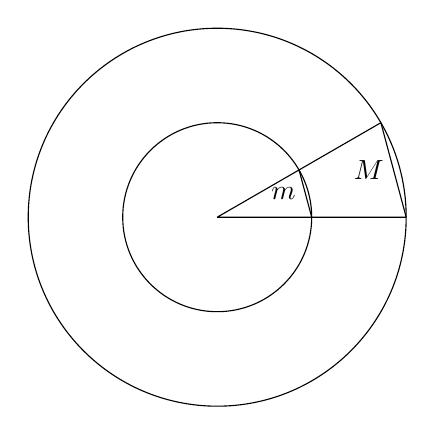
\begin{tikzpicture}[scale=0.6]
      \coordinate(O) at (0,0);
      \coordinate(A1) at (0:2);
      \coordinate(A2) at (0:4);
      \coordinate(B1) at (30:2);
      \coordinate(B2) at (30:4);
      \draw(O) circle(2) circle(4);
      \draw(O)--(A2) (O)--(B2) (A1)--(B1) node[midway,left]{$m$} (A2)--(B2) node[midway,left]{$M$};
      \tkzDrawPoints(O,A1,A2,B1,B2);
      % \draw[<->](0,-.2)--(2,-.2) node[midway]{$r$};
      % \draw[<->](0,-1)--(4,-1) node[midway]{$R$};
    \end{tikzpicture}
  \end{center}
  如上图,任意两个圆,若其半径相同,则圆周与直径的比值显然相同。考虑两圆半径不相同的情况,记小圆半径为$r$,圆周长为$c$;大圆半径为$R$,圆周长为$C$。将两圆圆心重叠放置,用如图中的折线逼近圆周,考虑其中一个折线段的比值,由三角形的相似性可以得到
  \begin{align*}
    \frac{m}{M} = \frac{r}{R}
  \end{align*}
  从而用折线近似的圆周比值也是
  \begin{align*}
    \frac{c}{C}=\frac{r}{R} \quad \implies \quad  \frac{c}{r} = \frac{C}{R}
  \end{align*}
  即其周长与半径的比值相同,从而其周长与直径的比值相同,其比值与圆的半径无关,是一个常数,通常记为$\pi$。并且通过下图可以估算出$\pi$的一个下界。
  \begin{center}
    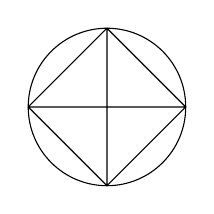
\begin{tikzpicture}[scale=1.0]
      \draw(0,0)circle(1);
      \draw(-1,0)--(1,0) (0,-1)--(0,1) (-1,0)--(0,-1)--(1,0)--(0,1)--(-1,0);
    \end{tikzpicture}
  \end{center}
  记上图中圆的直径为1,则其周长为$2\pi$,图中正方形的周长为$4\sqrt2$。两点间直线段长度最短,从而圆4个圆弧长度都要大于正方形的一条边长,由此可知圆的周长要大于正方形的周长,从而有
  \begin{align*}
    \pi>2\sqrt2\approx 2.8
  \end{align*}
  若将正方形换为内接正六边形,则可以得到$\pi$的另一个更精确的下界即$\pi>3$,参考例~\ref{ex:pww-3-lt-pi-lt-4}。事实上,古代人就是这样通过将圆不断的切割用更小的多边形来逼近得到$\pi$的近似值。
\end{proof}

\begin{example}
  $\pi$是无理数。但这个结论暂时还没有人能用简单或直观形象的方法得出,其多种证明无一例外都要用到更为高深的数学知识。此处不摘抄。
\end{example}

\subsection{自然对数底$e$}
\label{sec:irrational-number-e}

熟悉$e$的人都知道,$e$是自然对数的底。那么这个古怪的数是怎么来的呢?是数学家们凭空造出来提高门槛的吗?

实际上,$e$的出现比微积分还要早,它的产生与复利计息相关(可见经济问题也是推动科学发展的一大动力)。曾经有个商人向外放年利率是100\%的高利贷,即借出1元,一年后利息也是1元,一年到期后连本带利商人可以拿回2元。这是一年计息周期的。也有半年为计息周期的,即半年计一次利息,其利率为100\%的一半即50\%,计完利息后利息进入到下一个计息周期,对于半年为一个计息周期的情况,其计息结果如表~\ref{tab:e-compound-interest}所示,其中参与计息的本金是上期计息结算后利息与本金之和。
\begin{table}[htbp]
  \centering
  \caption{一年两次计息周期}
  \label{tab:e-compound-interest}
  \begin{tabular}{c|ccc}
    \hline
              & 参与计息的本金 & 利率 & 利息与本金之和\\\hline
    第一次计息 & 1             & 0.5 & $1 + 0.5$ \\
    第二次计息 & $1 + 0.5$     & 0.5 & $(1 + 0.5)^2$ \\
    \hline
  \end{tabular}
\end{table}

% 第一次计息时,参与计息的本金为1元,计息利率为$100\%/2=50\%$,计算出来的利息为$1\times 100\%/2=0.5$元,利息与本金这和为$1 + 1\times 100\%/2=1.5$元。

% 第二次计息时,参与计息的本金为上期的本金与利息之和即$1 + 1\times 100\%/2=1.5$元,计息利率仍然为$100\%/2=50\%$,计算出来的本金与利息之和为$(1 + 1\times 100\%/2)^2=2.25$元。

算到这里,商人发觉如果计息周期越短,计息期数越多,最终一年后连本带利能拿到的钱越多。发现了这个之后,商人兴奋了,如果以一秒钟为计息周期,那借1元出去岂不是就发大财了?

假设一年内分为$n$个计息周期,那么每个计息周期内的利率为$1/n$,一年后连本带利商人能拿回的钱$M$为
\begin{align*}
  M=(1+1/n)^n
\end{align*}
如果$n$无穷大,商人真的是能拿到无穷多的钱吗?利用计算机的帮助,举几个例子:
\begin{align*}
  n=&1       &&\implies M=2 \\
  n=&10      &&\implies M=2.5937424601\\
  n=&100     &&\implies M=2.70481382942153\\
  n=&1000    &&\implies M=2.71692393223559\\
  n=&10000   &&\implies M=2.71814592682493\\
  n=&100000  &&\implies M=2.7182682371923\\
  n=&1000000 &&\implies M=2.71828046909575\\
  n=&10000000&&\implies M=2.71828169413208
\end{align*}
结果可能要让商人失望了,当$n$趋于无穷大时,$M$是收敛于一个近似等于2.718的常数的,这个常数就是$e$,有时也称为欧拉数$e$(Euler数)、Napier常数。即
\begin{align*}
  e\equiv\lim_{n\to+\infty} \left(1+\frac1n\right)^n
\end{align*}

欧拉早在18世纪就证明了$e$是个无理数。他的证明是将$e$用形如$[2;1,2,1,1,4,1,1,6,1,\cdots,1,2n,1,\cdots]$的简单连分数表示出来。

\begin{question}
  $\pi + e$、$\dfrac{\pi}{e}$及$\dfrac{e}{\pi}$是否为无理数?这个问题,截止此文编写时({\the\year}年)仍然未有结论。
\end{question}

\begin{theorem}[欧拉公式,Euler Formula]
  \begin{align*}
  e^{ix}=\cos x + i\sin x
  \end{align*}
  取$x=\pi$,则可以得到连接了数学几个基本数字(虚数单位$i$、圆周率$\pi$、自然对数底$e$、1和0)的极为优美的一个恒等式:
  \begin{align*}
    e^{i\pi} + 1 = 0
  \end{align*}
\end{theorem}

\subsection{黄金比例}
\label{sec:irrational-number-golden-ratio}

黄金比例$\phi=\dfrac{\sqrt5+1}2\approx1.618$与$\Phi=\dfrac{\sqrt5-1}2\approx0.618$都是无理数,具体意义参考第~\pageref{ch:golden-ratio}页第~\ref{ch:golden-ratio}章。

类似于$\sqrt2$是无理数,$\sqrt5$也是无理数,从而由定理~\ref{th:rational-number-field}可知$\Phi$是无理数。

\section{代数数与超越数}
\label{sec:algebraic-number-and-transcendental-number}

\begin{definition}[代数数,Algebraic Number]
  若一个实数或复数是某个一元整数系数非零\footnote{非零是指方程的系数不全为零。}方程的根,则此数称为代数数。
\end{definition}

\begin{definition}[超越数,Transcendental Number]
  若一个实数或复数不是代数数,则称其为超越数。
\end{definition}

显然,有理数都是代数数,超越数必定是无理数。反之,无理数也有可能是代数数。

\begin{example}
  $\sqrt2$与黄金比例$\Phi$都是代数数。
\end{example}
\begin{proof}
  $\sqrt2$是整系数方程$x^2-2=0$的根,所以$\sqrt2$是代数数。

  可以利用下面的过程找到$\Phi$为其中一个根的整系数方程。
  \begin{align*}
                         &\Phi=\frac{\sqrt5-1}{2}\\
    \text{去分母}\implies &2\Phi=\sqrt5-1\\
    \text{有理数与无理数分类}\implies &2\Phi+1=\sqrt5\\
    \text{平方去根号}\implies &\left(2\Phi+1\right)^2=5
  \end{align*}
  由此可得$\Phi$是整系数方程$\left(2x+1\right)^2=5$的一个根。
\end{proof}

\begin{example}
  $\sqrt2+\sqrt3$是代数数。
\end{example}
\begin{proof}[提示]
  记$x=\sqrt2+\sqrt3$,则
  \begin{equation*}
    \begin{gathered}
      x^2=2+3+2\sqrt2\sqrt3=5+2\sqrt6\\
      x^2-5=2\sqrt6\\
      \left(x^2-5\right)^2=24
    \end{gathered}
  \end{equation*}
  由此可知$\sqrt2+\sqrt3$是代数数。
  若已有代数论中的域的知识,则有更为简单的方法。由于代数数在通常的运算规则下是一个域,而$\sqrt2$与$\sqrt3$都是代数数,从而其和也是代数数。
\end{proof}

\begin{theorem}
  有无穷多个超越数,且超越数组成的集合是不可数的。
\end{theorem}
\begin{proof}[提示]
  考虑实数的情况。这里用到了集合论里的可数与不可数概念,可以粗略地认为若一个集合不可数,那么它的元素个数比所有整数或者所有有理数的个数还要多\footnote{在集合论中,整数虽然是有理数的一个真子集,但其元素个数却是是一样多的,这是无限集与有限集的一个重要区别。}。其中一个简单的结论是整数组成的集合以及有理数组成的集合都是可数,实数组成的集合是不可数的。由于整数集是可数的,整系数一元方程的集合也是可数的,由这些方程的根组成的集合也是可数的,即代数数是可数的。因为两个可数集合的并集还是可数的,然而代数数与超越数的并集是实数集是不可数的,又已知代数数组成的集合是可数的,从而必有超越数组成的集合是不可数的。
\end{proof}

超越数是数学中较为纯粹的与生活无关的概念之一,通常只有数学家会对他们感兴趣。